\section{Auswertung}
\subsection{PV Wechselrichter}
\subsubsection{Wirkungsgrad Kennlinie}
Laut Datenblatt hat der Wechselrichter Sunny Island 2012/2224 im Betrieb, ohne Last, einen Eigenverbrauch von 21W. 
In unserem Fall lag der Eigenverbauch ohne Last bei 29,7 W. 
Der Eigenverbrauch wird dabei nach Formel \autoref{eq:230509_Eigenverbrauch} aus der Leistung am LR im Leerlauf bestimmt. 
Der Eigenverbrauch des Wechselrichters hat seine Ursachen dabei größtenteils aus den Schaltvorgängen, der in ihm verbauten Halbleiter, und den Ohmschen Widerständen.

\begin{equation}
	P_{ Eigenverbrauch }= U_{ LR} \cdot I_{ LR }
\label{eq:230509_Eigenverbrauch}
\end{equation} 


\begin{table}[!ht]
    \caption{test 1234}
	\centering
    \begin{tabular}{|l|l|l|l|l|l|l|l|l|l|l|l|l|l|l|l|}
    \hline
        Aufgabe & $P_{Sonne}$ & $U_{Gen}$ & $I_{Gen}$ & $U_{LR}$ & $I_{LR}$ & $I_{Batt}$ & $I_{WR}$ & $P_{AC}$ & $U_{AC}$ & $I_{AC}$ & f \\ \hline
        ${WR}_{allein}$ & 690 & 39,3 & 0,84 & 25,4 & 1,17 & 0,15 & 0,97 & 12 & 229,83 & 0 & 50 \\ \hline
        $Staub_{1}$ & 550 & 33,6 & 7,84 & 24,5 & 8,9 & -10,5 & 21,9 & 510 & 228,5 & 3,04 & 55;99  \\ \hline
        $Staub_{2}$ & 460 & 32,2 & 12,49 & 23,3 & 15,6 & -27,2 & 43,4 & 942 & 227,47 & 4,33 & 50;75 \\ \hline
        $Staub_{3}$ & 471 & 36,8 & 7,66 & 23,2 & 10,94 & -46,2 & 57,3 & 1208 & 226,98 & 5,05 & 50;67 \\ \hline
        SB-Heizung & 601 & 34,8 & 16,15 & 23,2 & 20,51 & -33,7 & 55,7 & 1186 & 227,4 & 5 & 50;56 \\ \hline
    \end{tabular}
	\label{tab:230512_Messtabelle}
\end{table}

Der Wirkungsgrad des Wechselrichters berechnet sich nach folgender Formel:
%
\begin{equation}
	\eta_{ WR} = \frac{ P_{AC} }{ P_{WR,Ein} }
	\label{eq:230509_Wirkungsgrad}
\end{equation}
%
%
\begin{figure}[!h]
		\centering
		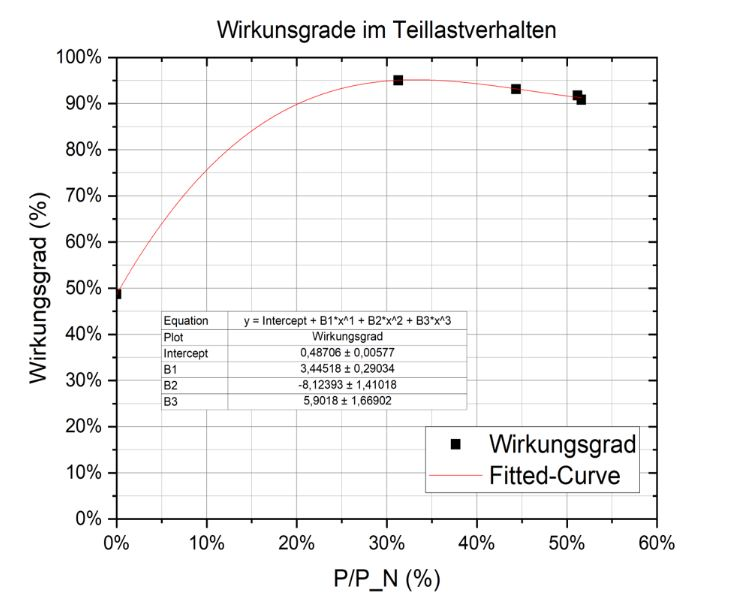
\includegraphics[width=0.7\textwidth]{Abbildungen/Kennlinie wr}
		\caption{Wirkungsgradkennlinie des Wechselrichters in Abhängigkeit der Auslastung}
		\label{fig:WRkennlinie}
\end{figure}
%
Dabei ist in \autoref{fig:WRkennlinie} zu erkennen, dass der Wirkungsgrad des Wechselrichters sich nicht linear verhält. Zunächst ist sehr niedrig und nähert sich dann einem Maximum an. Anschließend fällt der Wirkungsgrad wieder leicht ab, was an den steigenden Ohmschenverlusten liegt, die bei immer höher werdenen Strömen immer größer werden. Der maximale Wirkungsgrad liegt bei uns sogar bei 95 Prozent. Dies ist sogar 2 Prozent über dem Wirkungsgrad den der Hersteller angibt. Die ermittelte Kurve für den Wirkungsgrad ist dabei gut mit der Theorie zu vereinbaren. Des Weiteren ist zu erkennen, dass dieser Wechselrichter bereits ab 30 \% der Nennleistung sehr hohe Wirkungsgrade beseitzt, was ihn besonders gut macht für Standorte, die häufig Teilleistung liefern.
\subsubsection{Frequenz- und Spannungsstabilität}
Wie in unseren Messwerten zu sehen liegt die Spannung zwischen 226V und 230V. 
Die Spannung nimmt dabei mit steigender Leistung ab. 
Diese Werte passen auch sehr gut mit den Datenblattwert von 230 Volt zusammen. 
Die Frequenz bleibt dabei konstant bei 50 Hertz, wie man auf den Osziloskopbildern erkennen kann. 
Jedoch ist auch zu erkennen, dass der Sinus nur im Leerlauf und beim Anschließen der Straßenbahnheizung ohne Oberschwingungen daherkommt. 
Dies liegt daran, das hier ausschließlich Wirkleistung benötigt wird. 
Beim Anschließen des Staubsaugers erkennt man in \autoref{fig:oszi} die Oberschwingungen die entstehen. 
Dies liegt daran, dass der Staubsauer auch Blindleistung benötigt.
%
% \begin{figure}[!ht]
% 		\centering
% 		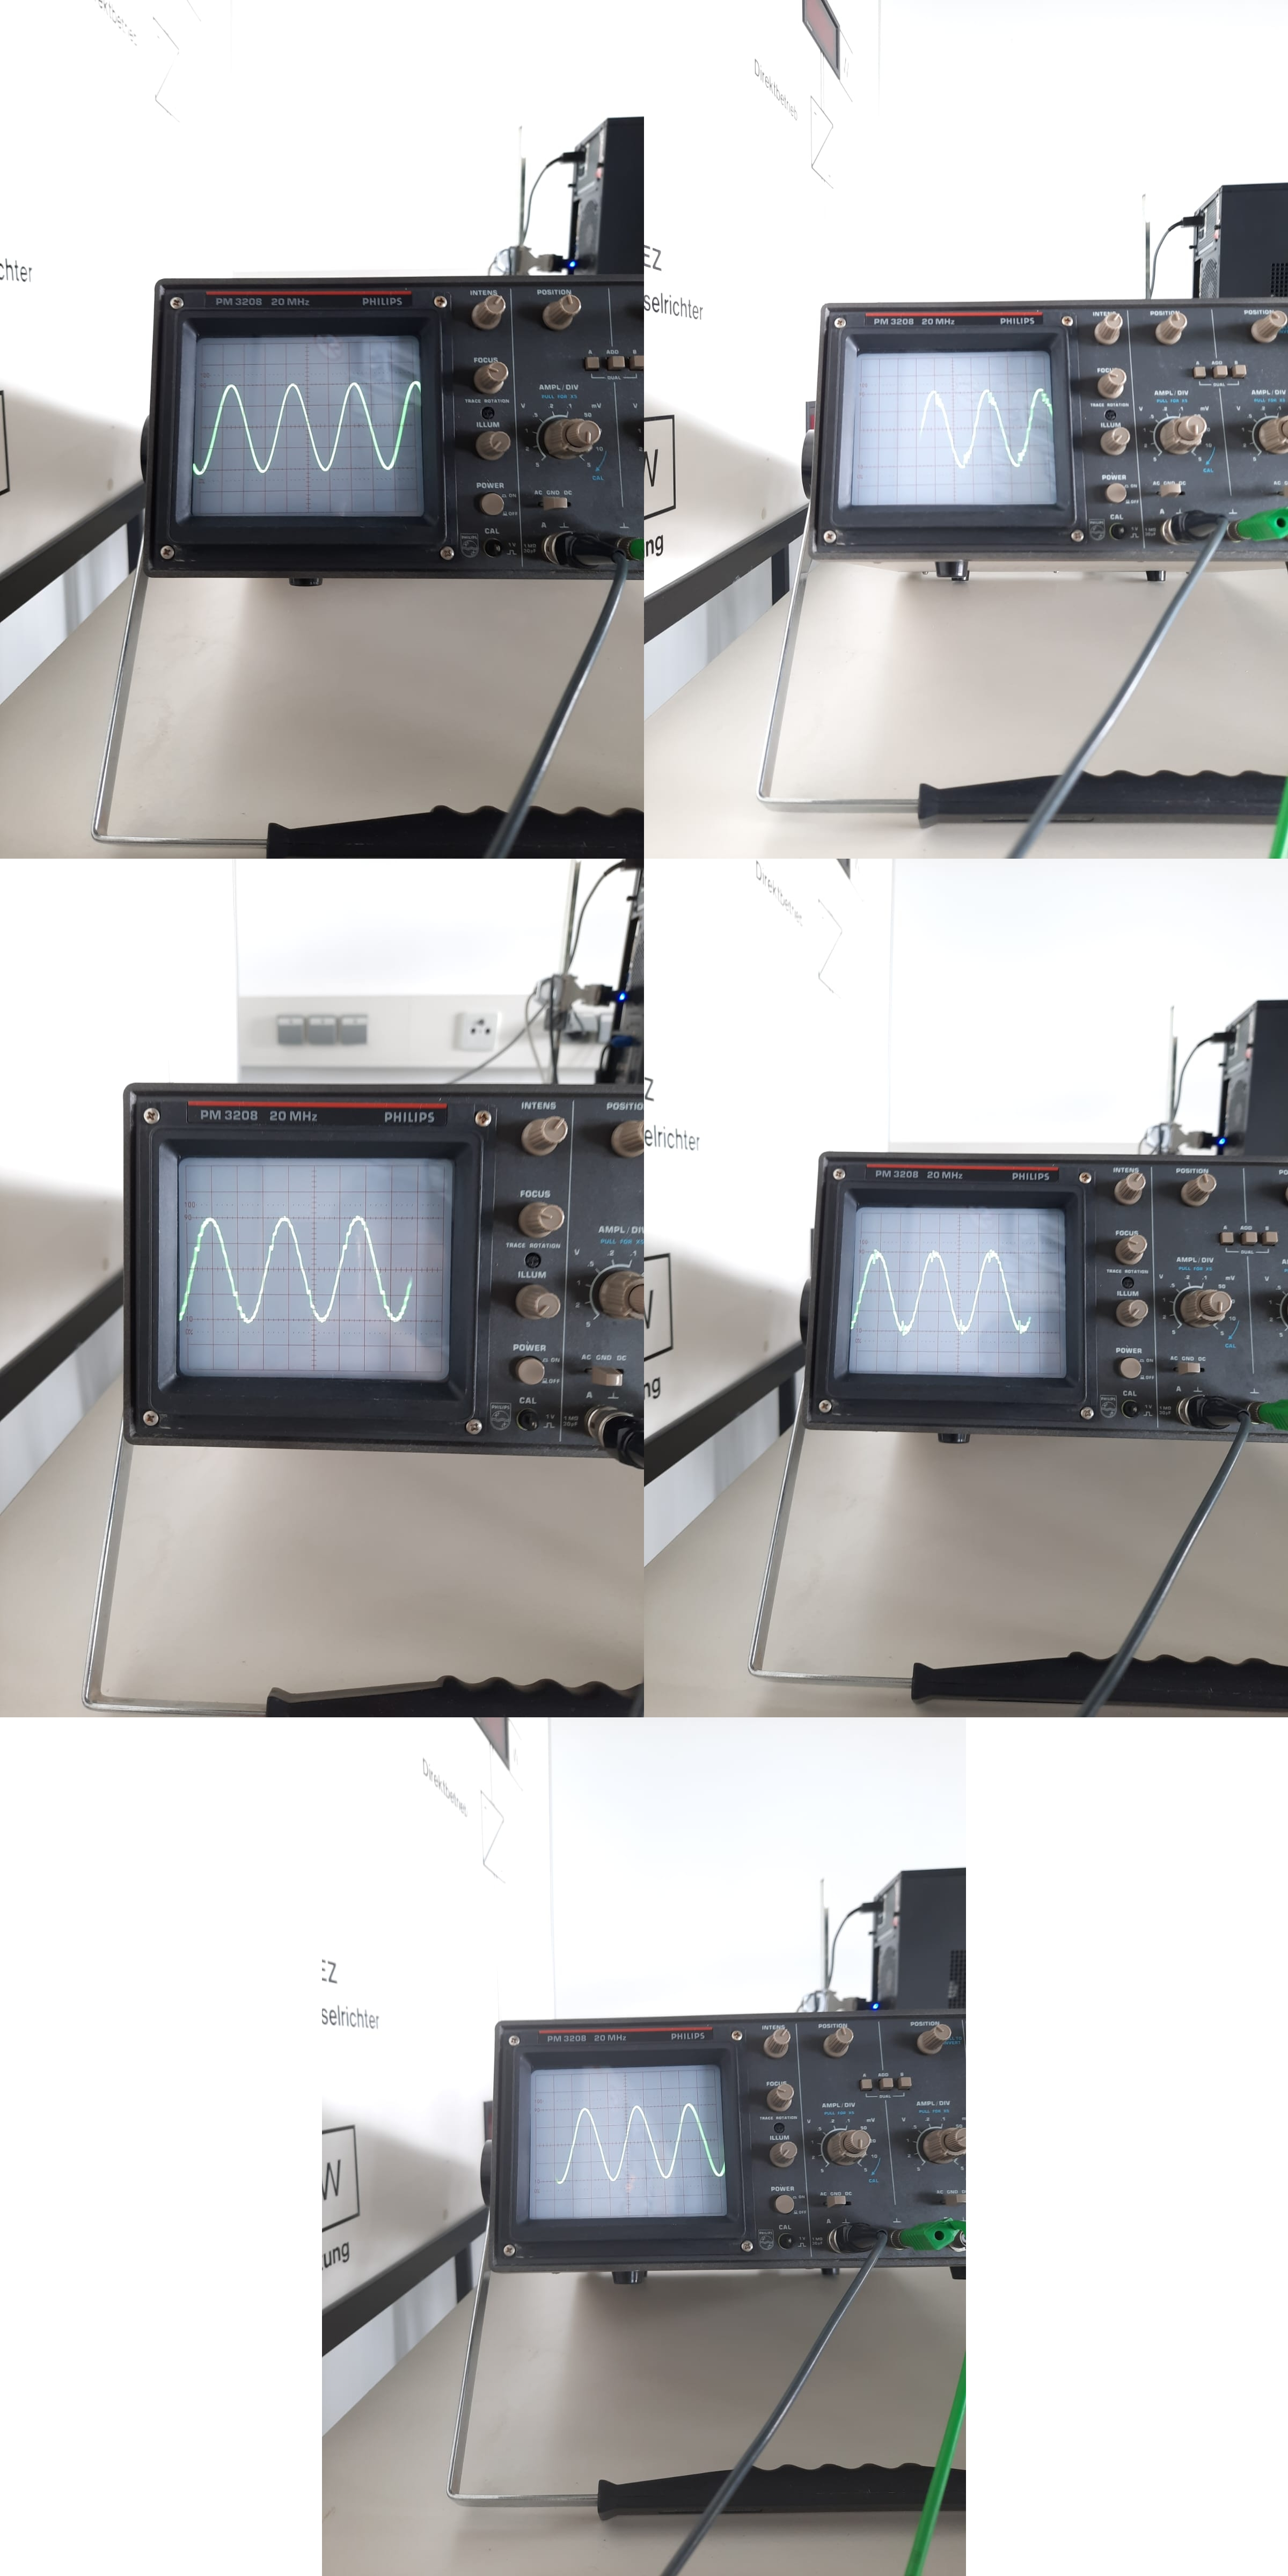
\includegraphics[width=0.5\textwidth]{Abbildungen/MergedImages}
% 		\caption{Von links nach rechts sieht man hier die Osziloskopbilder des Versuchs zuerst im Leerlauf, dann mit dem Staubsauger von Stufe 1-3 und im letzten Bild wurde die Straßenbahnheizung angeschlossen.}
% 		\label{fig:oszi}
% \end{figure}
%

\begin{figure}[H]
	\centering
	\begin{subfigure}[c]{0.19\textwidth}
		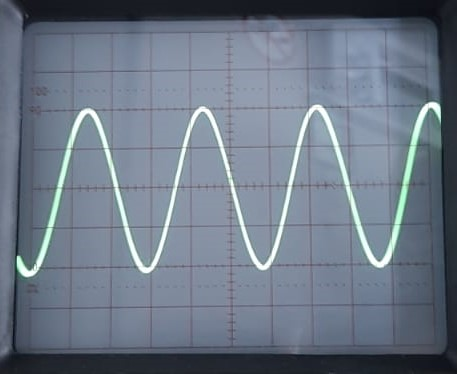
\includegraphics[width=\textwidth]{Abbildungen/Oszi_Leerlauf.jpg}
		\caption{Leerlauf}
	\end{subfigure}
	\begin{subfigure}[c]{0.19\textwidth}
		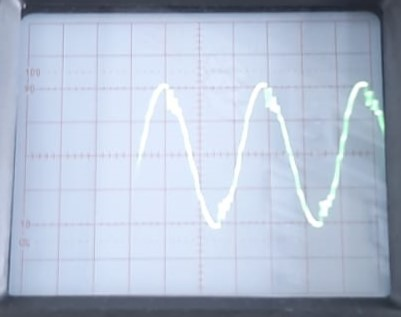
\includegraphics[width=\textwidth]{Abbildungen/Oszi_Staub_1.jpg}
		\caption{Staub 1}
	\end{subfigure}
	\begin{subfigure}[c]{0.19\textwidth}
		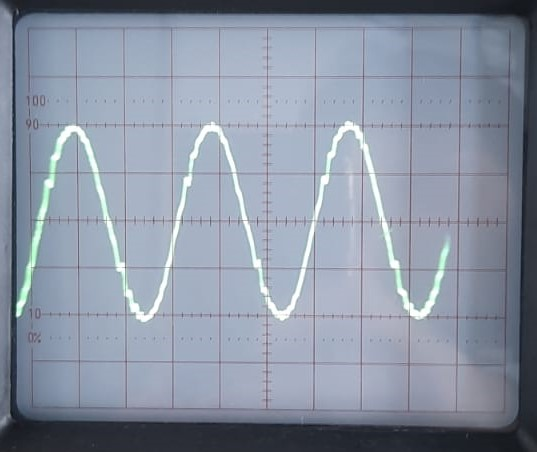
\includegraphics[width=\textwidth]{Abbildungen/Oszi_Staub_2.jpg}
		\caption{Staub 2}
	\end{subfigure}
	\begin{subfigure}[c]{0.19\textwidth}
		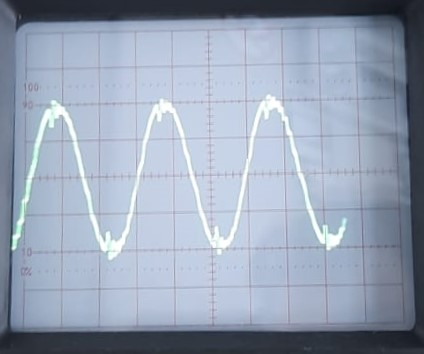
\includegraphics[width=\textwidth]{Abbildungen/Oszi_Staub_3.jpg}
		\caption{Staub 3}
	\end{subfigure}
	\begin{subfigure}[c]{0.19\textwidth}
		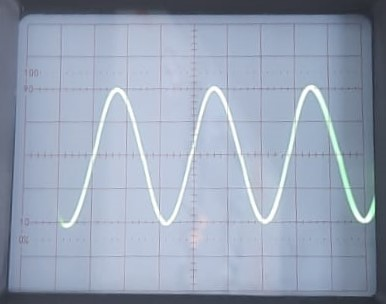
\includegraphics[width=\textwidth]{Abbildungen/Oszi_S-Bahn_Heiz.jpg}
		\caption{S-Bahn Heizung}
	\end{subfigure}
	\caption{Osziloskopbilder bei verschiedenen Leistungen}
	\label{fig:oszi}
\end{figure}


\subsubsection{Leistungsbeiwert}
Der Leistungsbeiwert $ \cos(\phi) $ berechnet sich nach \autoref{eq:230509_Cos(phi)}:
%
\begin{equation}
	\cos(\phi)=\frac{ P_{ AC,Wirk } }{  I_{ AC } \cdot U_{AC }}
	\label{eq:230509_Cos(phi)}
\end{equation}
%
Dabei ist in der Tabelle zu sehen, dass bei immer größerer Leistung beim Staubsauger Der Leistungsbeiwet sich immer näher an 1 annähert, was bedeutet, dass fast nur Wirkleistung benötigt wird. 
Leider ist es nicht möglich den Leistungsbeiwert anhand unserer Oszilosgramme zu bestimmen. 
Dies liegt daran, dass es nicht möglich war ein stehendes Bild zu erzeugen, anhand dessen es möglich wäre eine Aussage über den Phasenversatz zu machen. 
In der Theorie sollte mit steigendem Blindleistungsbedarf ein immer größer Phasenversatz zu sehen sein.